
\chapter{System Components}

This chapter will provide the explanation about the components of the system it and their attributes. It will also highlight how they intereact with each other in order to achieve the goals of this thesis. The chapter begins with explanation of profiling approaches, followed by impacts of context, critiquing and persuasion.

\section{User Profile}

One the core component of a system is to recommend user food that suits to his preferences, which can be gathered by profiling a user. In our system we followed a hybrid approach to build a user profile. Demographic information of a user is implicitly fetched from his Facebook account. The reason behind following implicit profiling approaches is to get user information without bothering them. This allows system to have up to date information about them.  However, it has been noticed that people are reluctant to those systems that request permission to access their social network activity information. Knowing these concerns, we only ask users to permit access to their basic information. Following are the acquired attributes from Facebook profile.

\begin{enumerate}
	\item Birthday
	\item Email	
	\item FirstName
	\item LastName
	\item Gender
	\item Name
	\item Profile Link
	\item UserId
\end{enumerate}

Moreover, explicit profiling techniques are used to gather users' contextual information and their preferences. While explicit profiling reveals accurate information, there however exist shortcomings in this technique. It demands user’s time and willingness to provide the data by filling the long forms, which seems to be tedious to the users. As the system is Knowledge based Personalized recommender, this problem has to be dealt efficiently because the recommendations produced by the system are highly influenced by user feedback. Therefore instead of making a user to provide all the information, we collect this data by using interactive forms based, which includes simple toggling, rating and selection mechanism that also increase the usability of the system.

\section{Food Profile}

Food recommendation is the basic research area of this thesis. Based on this approach our research is to provide recommendation according to both individual‘s dietary needs and preferences. Understanding food domain is very complex and challenging task when its come to recommender domain. User’s selection of a recipe is highly depends on it’s ingredients. Also there are some other factors which includes cooking methods, ingredient costs and availability, complexity of cooking, preparation time, nutritional breakdown, ingredient combination effects, as well as cultural and social factors \cite{freyne2010recommending}. Our research starts with in finding out how popular websites are dealing in this domain and structuring the recipes. So that we can get inspiration about the important features that user are looking for while he interacts with such system. Next chore of our research is to build a recipe database therefore we need a provider-API that ensures a large number of recipes. Among these APIs two notables with impressive meta-data about recipes are:

\begin{enumerate}
	\item Yummly API.
	\item BigOven API.	
\end{enumerate}

Both services are crowd-source driven, highly recommended in food domain and are offering almost the same data set. Next step to find the best suited API for our research therefore we preformed some experiments targeted to comparison between both selected API. Result of this experiment showed that Yummly API is not providing cooking description. On the other hand BigOven API doesn’t support recipe’s nutritional information and have limited number of calls per hour for student account. Regarding selection of API our focus was, it should provide all the relevant information about the recipes required by our research, in order to avoid any dependency. Considering mentioned fact we decided to choose BigOven API.\newline

Concerning about the attributes of food profile we followed the common approach that recipe have some important key attributes like cooking methods, ingredient preparation time, nutritional breakdown \cite{freyne2010recommending}.  However we are unable to get nutritional information due to API’s constrain, as discussed early, but in our data model we are considering it for future research purpose.  Figure \ref{fig:ch2_food_profile} illustrates the key attributes of food profile which is a common fashion for representing a recipe. We followed an hybrid approach \cite{suksom2010knowledge}
\cite{teng2012recipe} \cite{freyne2010recommending} for our personalize knowledge bases food recommendation system. Recipe’s ingredients are the primary factor on which recommendations are relied. 

\begin{figure}[h]
	\centering
	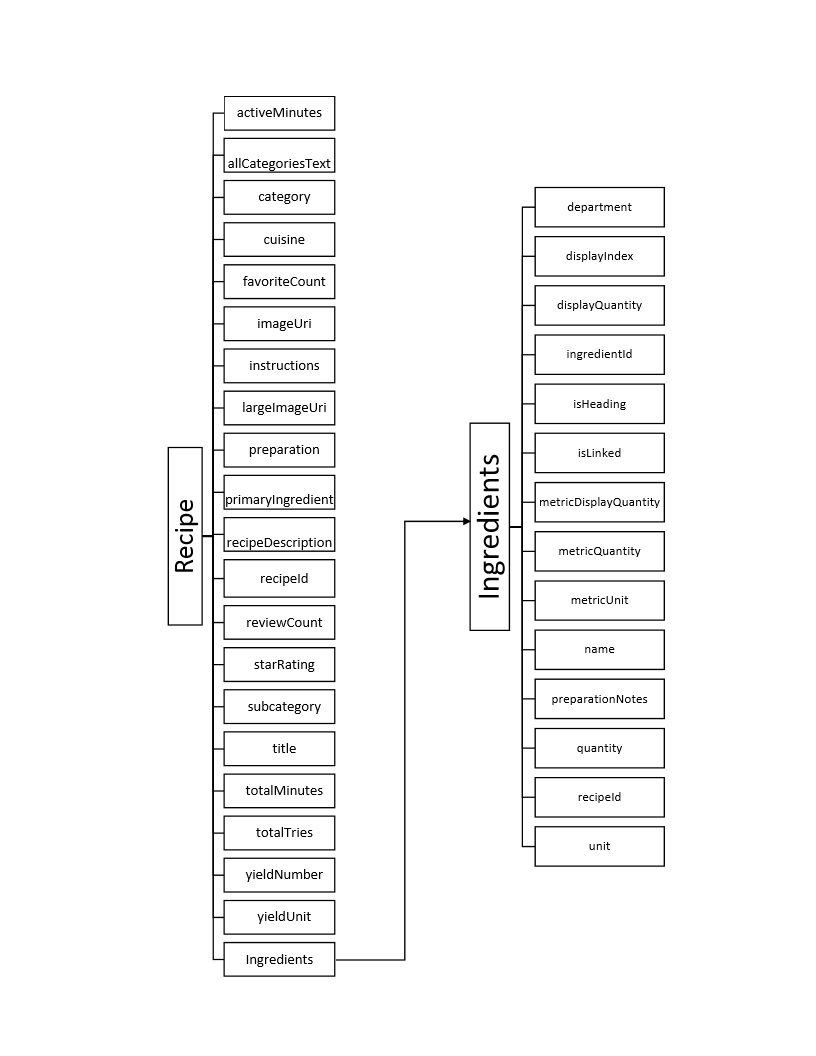
\includegraphics[width=.7\linewidth]{figures/ch2_food_profile.png}
	\caption{Attributes in Food Profile} 
	\label{fig:ch2_food_profile}
\end{figure}

\subsubsection{Assumption}

In order to simplify evaluation of recipe recommendation, System assumed that liking and disliking of ingredients by user is based on his dietary needs and health preferences. Suppose user does not like a particular ingredient let’s say “X”, therefore system learns from user’s critique and eventually avoids such recipes, which have "X" as an ingredient in it.

\subsubsection{BigOven API}

BigOven API provides all the information about the recipe in a well-structured and well documented manner. Along with the high number of recipes, they offer functionalities including  \textit{Search, Display Recipes, Recipe review, Grocery List and Rest-based API support}. For this thesis we focus only few of them to develop a database of your system.  Following are some API calls that are implemented in our system.


\begin{enumerate}
	\item \textbf{Reading a Recipe.}\newline \newline
	The Recipe object refers to a recipe within the BigOven collection.\newline \newline
%%%%%%% Request
	\textbf{URL request:}\newline 
	\textit{GET http://api.bigoven.com/recipe/{id}?api\_key="bigOvenApiKey"}
	\newline 
%%%%%%% Table	
	\begin{table}[ht]
		\centering % used for centering table
		\begin{tabular}{p{3cm} p{6cm} p{3cm}}  % centered columns (3 columns)
			\hline\hline %inserts double horizontal lines
			Parameter & Description & Required \\ % inserts table
			%heading
			\hline % inserts single horizontal line
			id & Primary key(ID) of recipe & Yes \\ 
			api\_key & Your api key issued to you by BigOven & Yes \\ 
			\hline %inserts single line
		\end{tabular}
		\caption{Bigoven- Reading a Recipe.}
		\label{table:bigoven-reading-recipe}
	\end{table}
%%%%%%% End Table		
	
	\item \textbf{Recipe Search Results.}\newline \newline
	The Recipe Search Result object is a collection of results for a given recipe search query.\newline \newline
	%%%%%%% Request
	\textbf{URL request:}\newline
	\textit{GET http://api.bigoven.com/recipes?title\_kw=" keyword"\&pg="page"\&rpp="resultPerPage"\\
	\&api\_key="bigOvenApiKey"	} \newline 
	
	%%%%%%% Table	
	\begin{table}[ht]
		\centering % used for centering table
		\begin{tabular}{p{3cm} p{6cm} p{3cm}}  % centered columns (3 columns)
			\hline\hline %inserts double horizontal lines
			Parameter & Description & Required \\ % inserts table
			%heading
			\hline % inserts single horizontal line
			title\_kw & Title keyword being searched for & No \\ 
			pg & Cureent Page to be fetched & No \\ 
			rpp & Number of results in page & No \\ 
			api\_key & Your api key issued to you by BigOven & Yes \\ 
			\hline %inserts single line
		\end{tabular}
		\caption{Bigoven-  Recipe Search Results}
		\label{table:bigoven-recipe-search-results}
	\end{table}
	%%%%%%% End Table	

\end{enumerate}

\section{Contexts}

Any information that can be used to characterized the situation of entity known as Context. For instance person, place\cite{ abowd1999towards}.  Incorporation of context in recommendation system leads to improve the quality of recommendation. System that uses context to provide relevant information is called context-awear system.  Lee, H. et al., \cite{lee2005context} classified context based on existing classification and definition in mobile domain. He categorized contextual information into five categories and further divided in to sub categories Figure\ref{fig:ch2_lee2005context} is a illustration of his classification.\newline 

\begin{figure}[h]
	\centering
	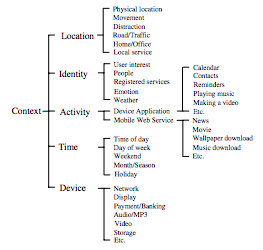
\includegraphics[width=.55\linewidth]{figures/ch2_lee2005context.png}
	\caption{Context hierarchy of the Mobile Web.} 
	\cite{lee2005context}
	\label{fig:ch2_lee2005context}
\end{figure}

\textit{Location} not only refers to user’s current location but also what objects are nearby to user such as destination, restaurants and local services. Also it tells about the state of the user like he is moving to staying with respect to specific place, such as home or office. \textit{Identity} is the representation of person’s interests e.g. emotional state, preferred keyword , usage history and social network. \textit{Activity} describe current usage of a mobile device,  for instance which services are using by user. \textit {Time} refers to  the current time as per system clock e.g. time of device, also time elaborates in terms of day, week, month of the year. \textit{Device} is a combination of hardware, software and network features that are provided by mobile for example Operating system version, Camera and Color.  Network explains as cellular technology and wireless interface such as 3G, LTE and Bluetooth.\newline
	
Considering Lee, H. et al.,’s classification\cite{lee2005context} as a foundation, different attributes of  context used in our system are discussed in the following forthcoming section.

\subsection{User Context}

As discussed in earlier section, user context create huge impact while recommendations are made.  Briefly, user context refers to the current activities of user. for example, what is the user during a specific circumstances. \textit{Cuisine’s Recipe and User Health and taste} are considered as  user interest in our system. User need to define \textit{ Cuisine’s Recipe} while he wants to interact with the system in order to narrow down the recommendation  according to selected food type. Since all the recipes are categorize as, drinks, breakfasts and appetizer.  Also \textit{User Health and taste}  context is gathered by user feedback. Considering user health and taste preferences system will not add those recipes, which do not matches to his profile. 
	
\subsection{Accessibility Context}
	
Accessibility context is a combination of “Activity” and “Time” according to above mentioned classification \cite{lee2005context}.  Following are the attributes which are related to our system: \textit{Cooking Time} indicates that how much time user have for cooking, so that system can recommend him only those recipes which are related to user’s preferred cooking time. \textit{Recipe’s Next Cooking Time} assume the recipe that user most likely to cook. System will not recommend the particular recipe which is already cooked by the user during a week. Assumption behind one-week cooking gap for a cooked recipe was to provide verity of recipes to user to maintain his interest. 
	
\subsection{Device Context}
	
Focus of this research is requires a mobile platform. Android, iOS and Windows phones are the three considered option. We selected iOS platform and chose iPhone as a selected device for developing our prototype. The reason behind the selection of iOS, was to develop a high fidelity UI which is intuitive and useable, by considering all the User interface guide lines provided by Apple Inc. iOS version that is required by our app is minimum 8.3. However, client side code written in swift programming language, highly recommended by Apple Inc.

\section{Critiquing}
Elicitation of user preference is the key step of recommendation system. There are many simple approaches for accusation of user preferences and transform it into user model. Traditionally, these were acquired explicitly where user need to fill a form and mentioned his wants and need. However, it has been noticed users avoid in filling information about themselves. Using these approaches result less knowledge about user preference and poor recommendations. To solve these problems two methodologies have been suggested. In first approach accusation of user’s preferences takes place by analyzing of user’s navigation behavior. This assumption that user always visit his interested item. Advantage is requiring lower user effort. While shortcomings are: (1) It depends understating of domain specific knowledge because user actions are translated into user preferences model. (2) Noise existence because preference and context of a person may differs from another person.\newline

Second is conversational approach a new paradigm for the collection of user preference and redefines human-computer interaction. Such systems are based on interaction cycles in order to gather preferences about the users. At interaction cycle, the system can either ask the user a preference or propose a product to the user. The user can reply either by answering to the question posed or by criticizing the system proposal.\cite{ricci2005critique}\newline

Moreover, Critiquing by conversational approach is not enough in our case. It can answer to the cold startup problem and are unable to deliver quick results. Therefore Active Learning (AL) is the additional approach, which is used by our system in order to quickly deliver good results without preexisting knowledge about user preferences. \cite{lamche2014active}. We followed Model-based AL methodology in order to construct user model regarding ingredient and recipe selection, avoid expected error in model. As far as AL mode is concerned we followed the Sequential model states as: recalculate the rating of item once user rated that specific item. In our case ingredients and recipe \cite{rashid2008learning}.

Following our goal to develop the user profile over time using active learning methods in recipe recommendation scenario. Training points of our application is recipe rating, ingredient like/dislike that will build over time in order to make accurate suggestion. Initially when we have no training point based on conversational approach our system recommends top ten recipes according to given contextual information based on Cuisine and Current Preferred cooking time of user. As it is unlikely that user always wish to eat same type of food and have same cooking time. At some point user have a tough schedule due to other activities and have less time to cook. Similarly eating preferences changes with respect to meal ‘s time like breakfast, lunch, dinner and drinks. Considering the dynamic behavior of user and interest conversational approach is more suited. We followed Knowledge based recommendation approach, as our system is more specific to user’s health and taste and the more knowledge about the user have more strong recommendation would be. We also consider content-based approach in our system in order to select popular recipes among the users to drag the attention of user. Initially when system does not have user preference, it follows collaborative filter approach by suggestion him top ten recipes of system. In order to improve the critiquing we are categorized in two manners, First, How much to like the recipe based on star rating. Second user likes particular ingredient or not which is Boolean in nature. Where system categories each ingredients in three state like, dislike and neutral (these are neither like nor dislike by user).  
	
\section{Persuasion}

\section{Approaches}
